\section{Modelo de iluminación}

\SectionPage

\begin{frame}{Normal de una isosuperficie}
    
    Para un modelo de iluminación es indispensable el cálculo de la normal de una isosuperficie, por ello, vamos a presentar el siguiente teorema:

    \begin{theorem}
        El vector gradiente \(\nabla f(x_0, y_0, z_0)\)  es perpendicular a la curva de la tangente de una \textit{isosuperficie} en el punto \(\Vec{p}=(x_0, y_0, z_0)\).
    \end{theorem}
    
    En realidad, nos quiere decir que la normal de una \textit{isosuperficie} es proporcional a su gradiente o exacta en caso de su posterior normalización:
    
    \[
        \Vec{n}=norm(\nabla f(x, y, z))\approx norm\left(
        \langle
        {\begin{array}{c}
        \dfrac{f(x+0.001,y,z)-f(x,y,z)}{0.001}\\
        \dfrac{f(x,y+0.001,z)-f(x,y,z)}{0.001}\\
        \dfrac{f(x,y,z+0.001)-f(x,y,z)}{0.001} \end{array}}
        \rangle\right)
    \]
    
\end{frame}


\begin{frame}{Intensidad lumínica}
    
    Para cada luz \(\Vec{l_i}\in L\), definimos el vector director de la luz hasta el punto \(\Vec{p}\) como  \(\Vec{d}_i=\text{norm}(\Vec{l_i}-\Vec{p})\), la intensidad es un factor multiplicativo.
    
    \vfill
    
    \begin{columns}[onlytextwidth]
        \begin{column}{0.30\textwidth}
            {\Large Intensidad ambiental}\\
            
            Intensidad mínima sobre la isosuperficie. 
            
            \vfill
            \begin{figure}[H]
              \centering
              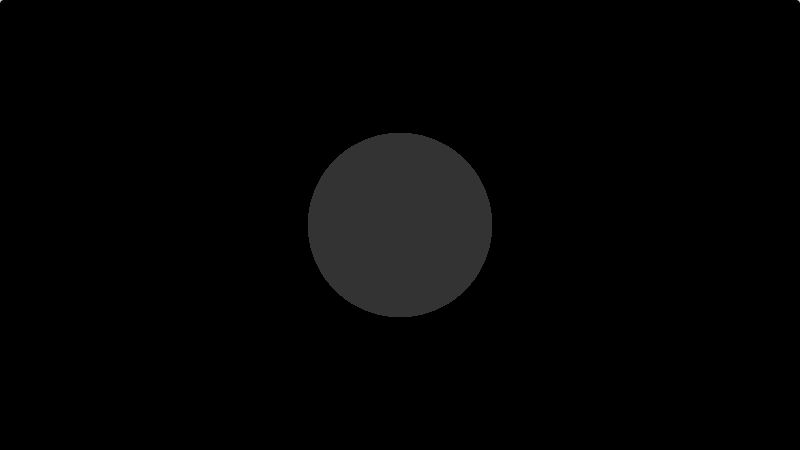
\includegraphics[width=1.0\textwidth]{imagenes/lightmodel/ambiental.png}
            \end{figure}
            
            \vfill
            \[I_a \in [0,1]\] 
        \end{column}
        
        \begin{column}{0.30\textwidth}
            {\Large Intensidad difusa}\\
            Intensidad por la luz refractada por la superficie.
            \vfill
            \begin{figure}[H]
              \centering
              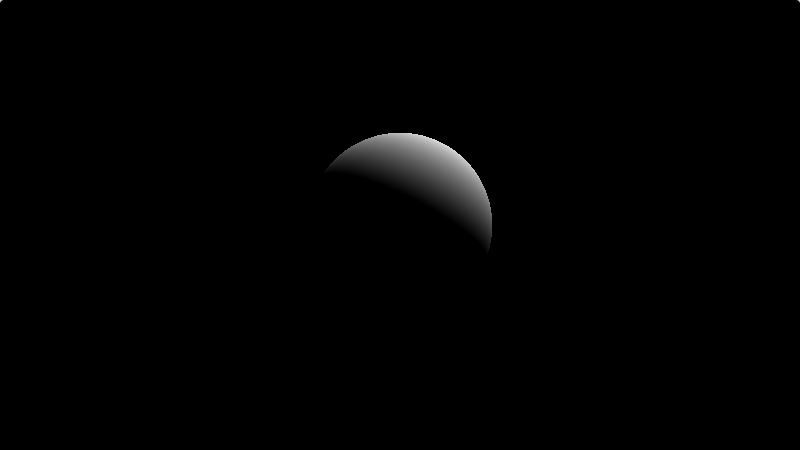
\includegraphics[width=1.0\textwidth]{imagenes/lightmodel/difusa.png}
            \end{figure}
            \vfill
            \[I_d = \sum_{\Vec{l_i}\in L} \Vec{n}\cdot\Vec{d_i}\]
        \end{column}
        
        \begin{column}{0.30\textwidth}
            {\Large Intensidad especular}\\
            Intensidad por la incidencia en el ojo de la luz reflectada.
            \vfill
            \begin{figure}[H]
              \centering
              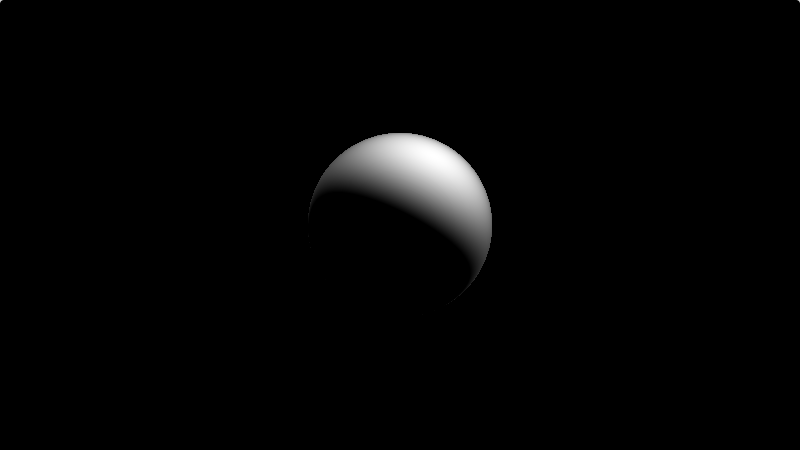
\includegraphics[width=1.0\textwidth]{imagenes/lightmodel/especular-0.png}
            \end{figure}
            \vfill
            \[I_e = \sum_{\Vec{l_i}\in L} \Vec{ojo}\cdot\left(\Vec{d_i} \veebar \Vec{n}\right)\]
        \end{column}
        
    \end{columns}
    
\end{frame}


\begin{frame}{Modelo de Iluminación de Phong}

    Presentado por Thuong Phong en 1975 como un modelo empírico, resultado de las sumas de las intensidades anteriores, además, utiliza un \textit{homeomorfismo} como factor de brillo para la intensidad especular:
    \[h_k:[0,1]\longrightarrow[0,1] , h_k(x)=x^{2^k}\]
    \[I_{Phong}=I_a+\sum_{\Vec{l_i}\in L} \mathrlap{\underbrace{\phantom{\Vec{n}\cdot_{[0, 1]}(\Vec{l_i}-\Vec{p})}}_{\text{Intensidad Difusa}}}\Vec{n}\cdot_{[0, 1]}(\Vec{l_i}-\Vec{p}) + \mathrlap{\underbrace{\phantom{h_k\left(\Vec{ojo}\cdot_{[0, 1]}\left(\left(\Vec{l_i}-\Vec{p}\right) \veebar \Vec{n}\right)\right)}}_{\text{Intensidad Especular}}}h_k\left(\Vec{ojo}\cdot_{[0, 1]}\left(\left(\Vec{l_i}-\Vec{p}\right) \veebar \Vec{n}\right)\right)\]
    
    \begin{figure}[H]
      \centering
      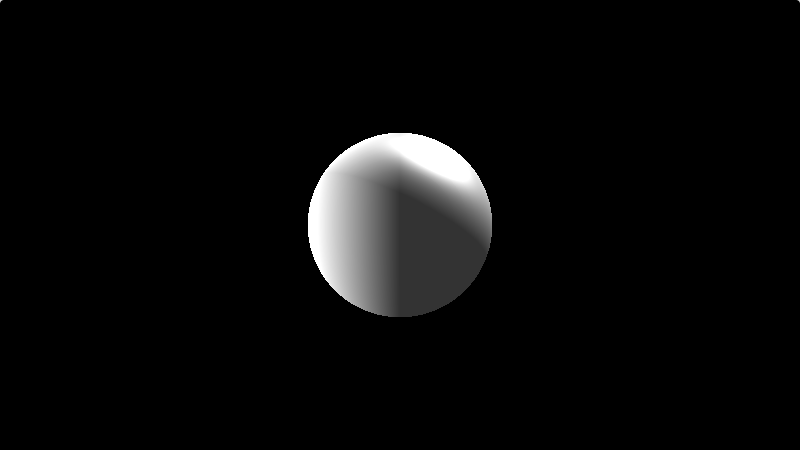
\includegraphics[width=0.5\textwidth]{imagenes/lightmodel/phong.png}
    \end{figure}
    
\end{frame}

\begin{frame}{Umbra}

    Dado un punto punto \(\Vec{p}\) sobre la superficie, lanzaremos otro rayo hacia la luz para ver si este es ocluido, en caso de trazar otro punto \(\Vec{q}\) en esa dirección, la intensidad se mantendrá constante.
    \vfill
    Al lanzar el rayo desde la una isosuperficie, las primeras iteraciones resultan de bolas pequeñas, por ello, separaremos el punto \(\Vec{p}\) de la superficie haciendo uso de la normal de la superficie y un factor de empuje \(k\in\mathbb{R}^{+}_{0}\).
    \[\Vec{p'}=\Vec{p} + \Vec{n} \cdot k\]
    \vfill
    \begin{figure}[H]
      \centering
      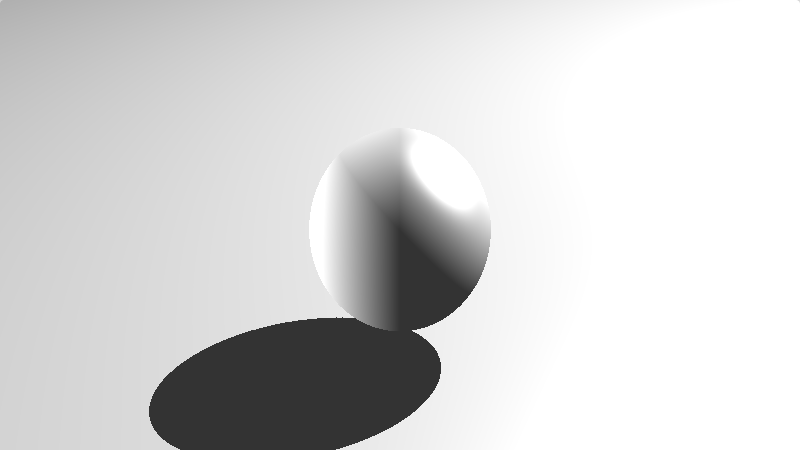
\includegraphics[width=0.5\textwidth]{imagenes/lightmodel/sombra_dura.png}
    \end{figure}
    
\end{frame}